\documentclass{article}[10pt]
\usepackage{graphicx}
\usepackage{xspace}
\usepackage{url}
\usepackage{listings}
\usepackage{color}

\definecolor{pblue}{rgb}{0.13,0.13,1}
\definecolor{pgreen}{rgb}{0,0.5,0}
\definecolor{pred}{rgb}{0.9,0,0}
\definecolor{pgrey}{rgb}{0.46,0.45,0.48}

\lstset{language=Java,
  showspaces=false,
  showtabs=false,
  breaklines=true,
  showstringspaces=false,
  breakatwhitespace=true,
  commentstyle=\color{pgreen},
  keywordstyle=\color{pblue},
  stringstyle=\color{pred},
  basicstyle=\ttfamily,
  moredelim=[il][\textcolor{pgrey}]{$$},
  moredelim=[is][\textcolor{pgrey}]{\%\%}{\%\%}
}

\newcommand{\lstJava}[1]{\lstinline[language=Java,breaklines=true,mathescape,literate={\-}{}{0\discretionary{-}{}{}}]�#1�}
\newcommand{\tapcli}{Tapestry5-cli\xspace}

\begin{document}

\title{\tapcli Library}
\author{Alessio Gambi}

\maketitle

\begin{abstract}
This document briefly describes the design process that I followed while implementing the \tapcli library.
The idea is to illustrate over a real example how to design new services by using Tapestry 5, and ideally, start sketching a generic process to develop Tapestry5-driven applications.
\end{abstract}


\section{Introduction}
This document is not meant to be a user guide for the library. The document contains in a somehow organized fashion the various concepts that I encountered during the design of a simple library, i.e., \tapcli.
During the development I was advised by two members of the Tapestry 5 community, Thiago and Barry, that provide useful suggestions and insights.

\section{The Problem}
We need to parse the command line input of our Java program following user specifications, check the validity of provided values according to user specified constraints, and finally, make the various options and inputs available to the application.
If parsing or validation fail we throw an exception, and print on the console an error message that describes what failed and why, and we also print a usage message that described the correct syntax of expected by out application.

Ideally, all the messages must be localized; furthermore, error messages must be as specific as possible, and the usage message must list all the available options and constraints.

In the spirit of Tapestry 5, we want to configure the library in a distributed fashion:
Several modules can contribute their own input options, and configurations; validation mechanisms, messages, and all the other contributions can be specified as well in the modules.

\section{Solution Overview}
We want to exploit the full power of Tapestry5-IoC to design a library that provides a service, called \lstJava{CLIParser}, which implements parsing and validation of the command line input, on one side, and exports options, their values, and the other application inputs as \lstJava{Symbols}.

\begin{figure}[h!]
 \centering
  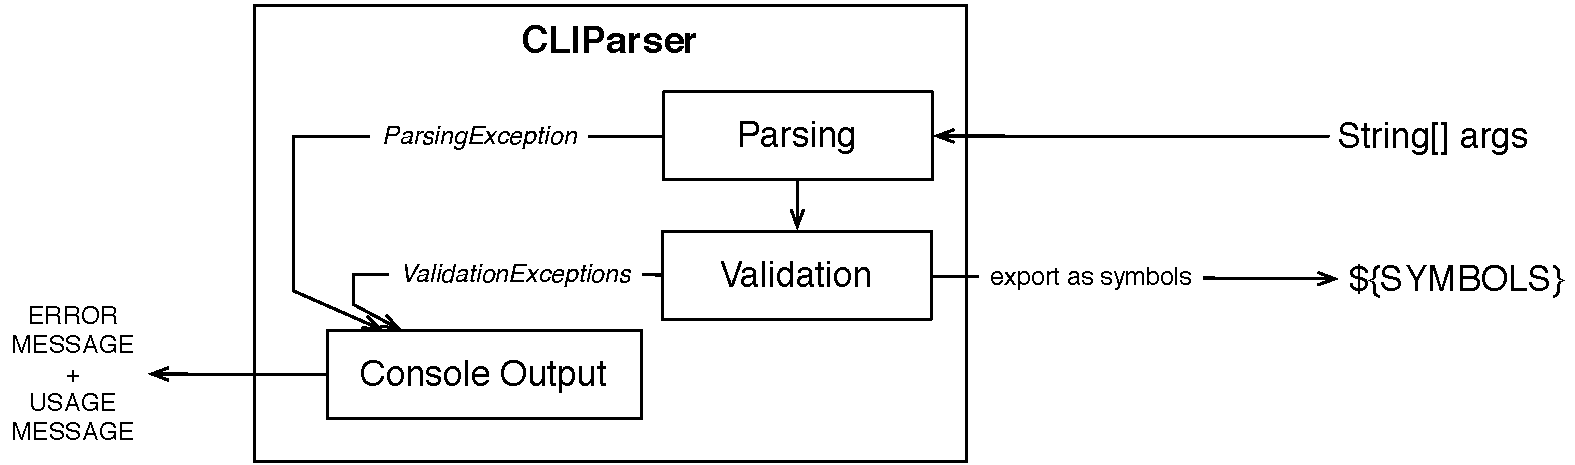
\includegraphics[width=0.8\textwidth]{figs/overview.pdf}
  \caption{Overview of the \tapcli library}
  \label{fig:overview}
\end{figure}

Figure~\ref{fig:overview} depicts an informal overview of the solution.
The \lstJava{CLIParser} receives the input arguments, try to parse them using some {\em Parsing} logic that is pipelined with the {\em Validation} logic. 
If the parsing succeeds the control passes to the validation code, otherwise a \lstJava{ParsingException} is raised and the pipeline breaks. Similarly, if the validation succeeds the control pass over, otherwise a \lstJava{ValidationException} is raised and the pipeline breaks. 
If an exception is raised, the \lstJava{CLIParser} must generate useful messages for the user and print them on the Console, as this is the common behavior that we expect from applications that are started using the command line.
If no exceptions are thrown, the \lstJava{CLIParser} exports the validated inputs as \lstJava{Symbols} to be accessed elsewhere by our Tapestry-IoC enabled application.

In implementing the library the general suggestion is to exploit as much as possible the functionalities provided by Tapestry5, and Tapestry5-modules provided by third parties; however, we can also use third party libraries for any basic/generic functionality that we need and that Tapestry5 does not yet  provide. For example in our case, we use the {\tt commons-cli} library provided by Apache\footnote{\url{http://commons.apache.org/proper/commons-cli/}} to implement the functionalities for parsing the CLI.
Of course, any third party library that we use must be seamlessly integrated with the other Tapestry5 provided services and the Tapestry5-IoC framework.

\paragraph{Distributed configuration}
We rely on the distributed configuration feature of Tapestry5 to collect all the user-provided configurations to properly configure the third-party libraries and the other services. We may need to collect information about the allowed parsing options and switches, e.g. what characters can be used and for which option, but also constraints to check if the provided input values are valid, e.g., the second input is a \lstJava{String} and its length should be less than ten characters but more than two.

In the simplest case, we can have that all these informations are in the \lstJava{AppModule} of our application. In fact, it is reasonable to follow the {\em locality principle} and put all the informations about a concept close to it; in our terms this means that we want to specify which inputs are allowed, and what are their validation constraints in the same place, i.e., the \lstJava{AppModule} class, where we {\em build} the services that depends on such configurations. 

The left side of Figure~\ref{fig:distributed} shows a simple example, where we build a service {\tt Foo} that expects four inputs, namely, {\it alpha}, {\it beta}, {\it gamma}, and {\it repetitions}. In the same module, we specify also that we allow four options (one for each of these inputs) to be specified on the command line\footnote{Note that as they are accessed as symbols we can also pass the inputs defining system properties, environmental variables, configuration files an so on}. With the definition report in the figure, we are constraining the users of our application to provide inputs according to the following pattern\footnote{Note that the input order does not count}:
use {\tt -a} (or {\tt -}{\tt-alpha} followed by one input argument, 
use {\tt -b} (or {\tt -}{\tt-beta} followed by one input argument, 
use {\tt -g} (or {\tt -}{\tt-gamma} followed by one input argument,
and finally, use {\tt -r} (or {\tt -}{\tt-repetitions} followed by one input argument.

In the general case, we may use multiple modules at the same time, and each of them may need to specify its own set of options. Therefore, we need to collect and manage in a consistent fashion all these options. For example, we may need to check that an option is not defined twice, or its accessed but never defined. Moreover, we may need to consider that modules can contribute additional validations logic, messages, and so, that must be mixed together at startup time. This situation is exemplified in Figure~\ref{fig:distributed}.
\begin{figure}[h!]
 \centering
  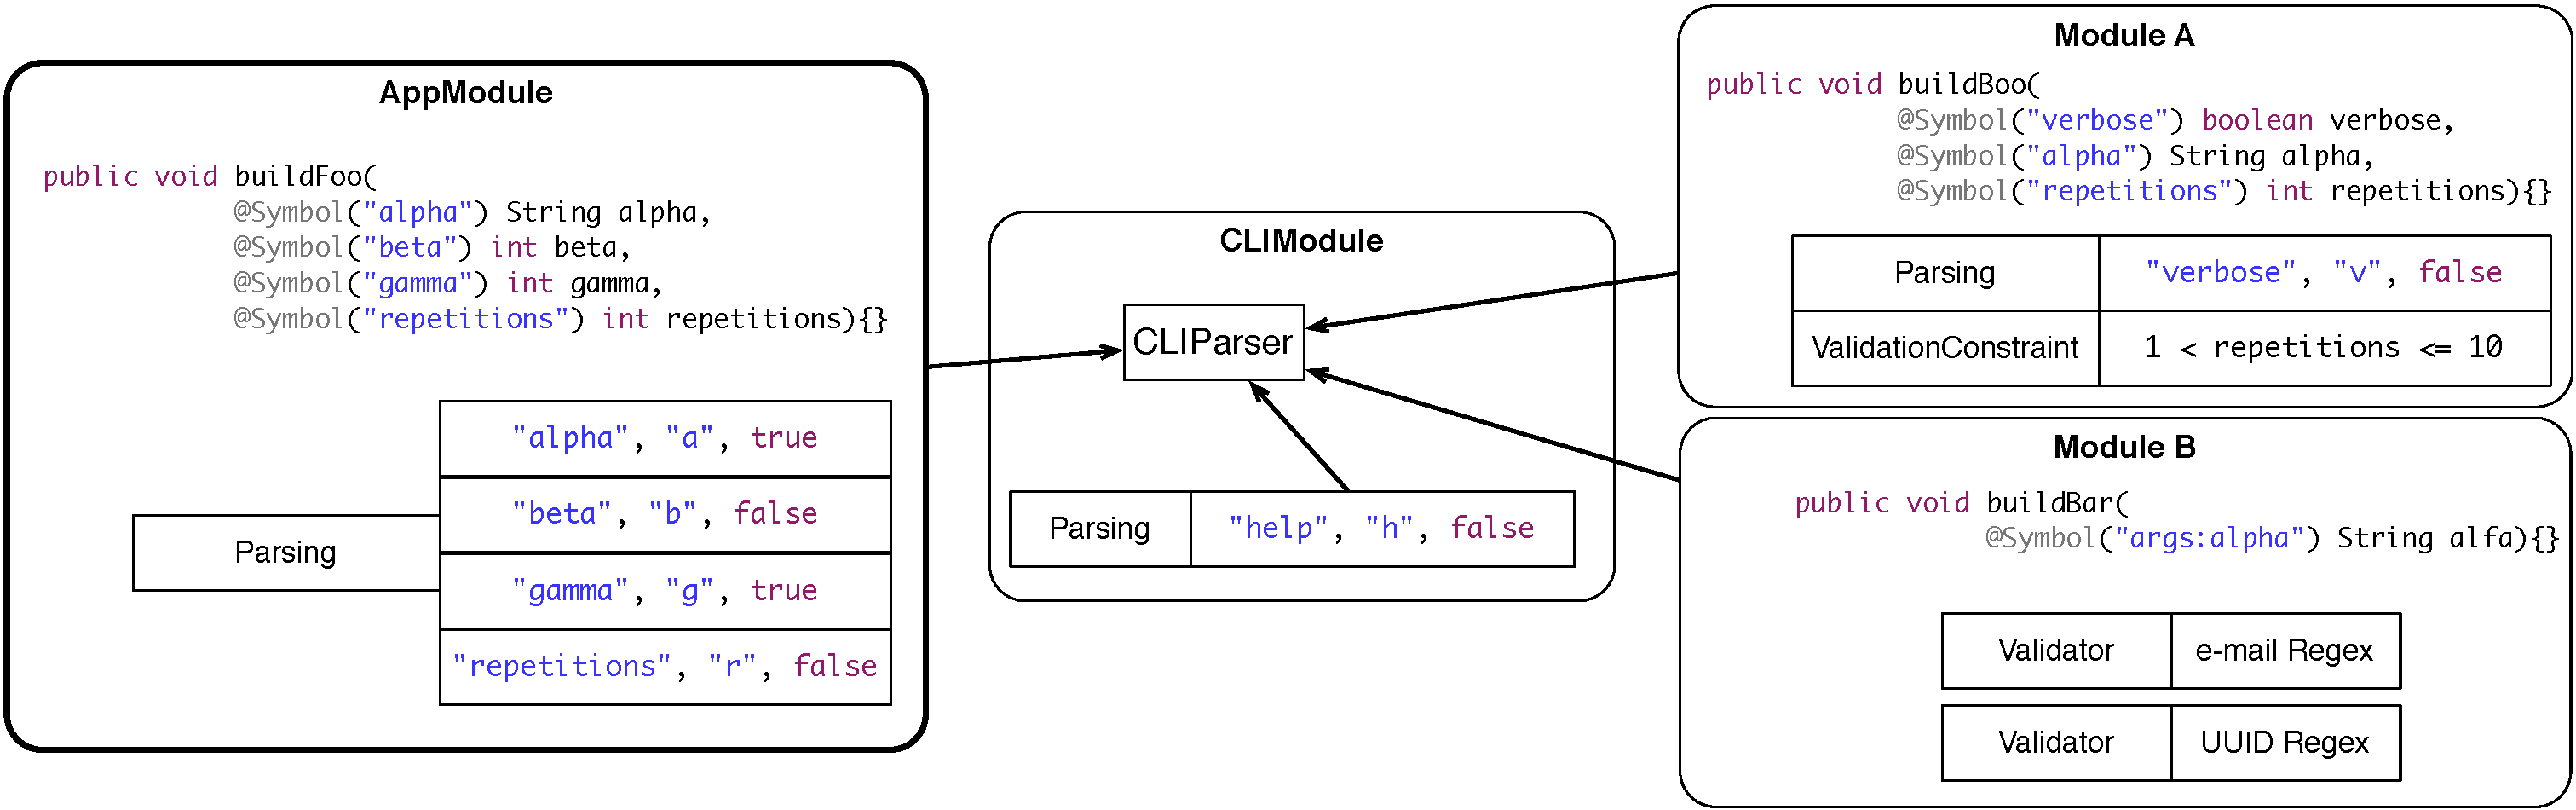
\includegraphics[width=\textwidth]{figs/distributedconf.pdf}
  \caption{Distributed configuration of \tapcli}
  \label{fig:distributed}
\end{figure}

\subsection*{Architectural considerations and design alternatives}
Considering the common patterns promoted by Tapestry5 and the description of the solution overview, we found that a possible design pattern (or combination of patterns) that we can adopt is the {\em Chain-of-Command}:
A possible chain can be defined by the {\em terminator} command that is export all the input arguments, parsed options and their values as \lstJava{Symbols}, that is preceded by the Validation command, and the parsing command (see the inner diagram of Figure~\ref{fig:highlevelarchitecture}).

\begin{figure}[h!]
 \centering
  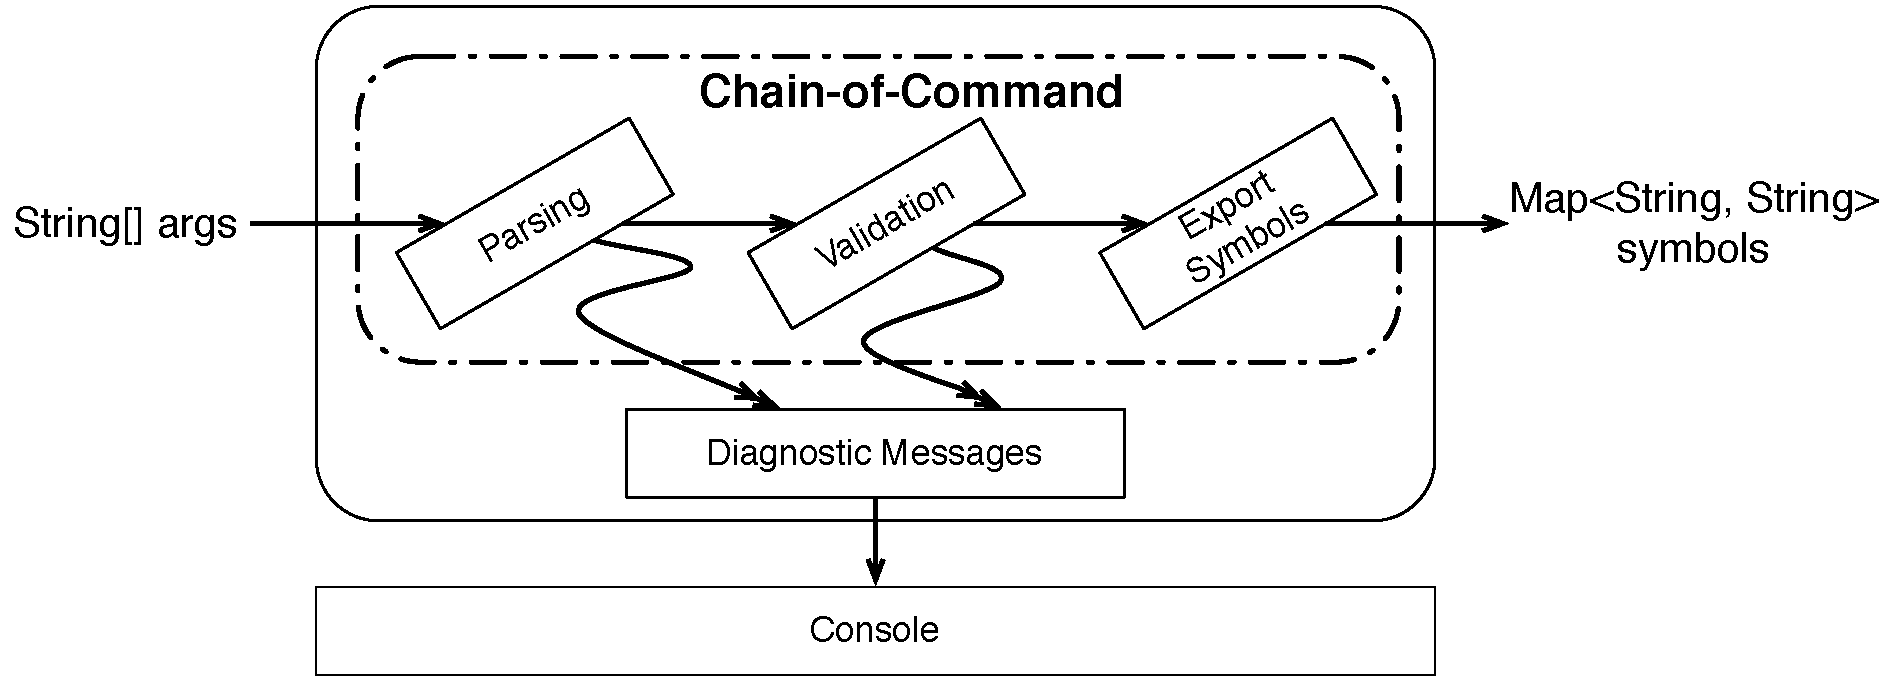
\includegraphics[width=\textwidth]{figs/highlevelarchitecture.pdf}
  \caption{High level architecture of the \lstJava{CLIParser} service}
  \label{fig:highlevelarchitecture}
\end{figure}

The chain let us realize a subset of the required functionalities, in fact we can realize the {\em positive} scenario provided that we input a well formed input on the command line, and provided the all the values are valid. However, we cannot yet realize the {\em negative} scenario, that is, the generation on the output of the diagnostic messages and the usage message in case the provided input is not well formed or some of the input values are not valid. 
% TODO: Here I feel something is missing
To do so we need to wrap the inner chain with proper code to capture the exceptions, create the contextualized message for the user, print that out to the console, and finally, stop the application execution.


With this information we identified some possible solutions to be evaluated:

\begin{description}

\item[Mock Up Requests] We can mock up the startup process as the process of a single Web request to the framework, and exploits as much as possible the services already available in the framework, as well as their organization. This has the pros to have basically everything in place, but has the cons of not using the framework in the right wait. It also is quite an "hacky" solution, that may bring in a lot of problems to bend the framework to our needs. Moreover, if we follow this solution, we will end up having a lot of code and dependencies that we do not really need.

\item[Create a clone of the  Request Pipeline] Another way to reuse as much as possible the services already defined is to recreate the main pipeline request process. In this way, we can choose what service to put inside the pipeline processing and we limit the `hacking' of having a non-web request processed as a web-one. Differently from the previous we just provide a special request in input and let it be processed by the framework. Still this solution is quite ``hacky'', but has the pros to allow a direct use of the \lstJava{Messages}, \lstJava{TranslatorSource}, and \lstJava{Validator}. As a matter of fact at the time of writing Tapestry5 provides implementations of these services\footnote{Messages technically is not a service but it can be managed the same way} only in the Web part.

\item[Use ChainBuilder and define our own chain] Instead of replicating tapestry code we can build the services that we need and organized them by leveraging \lstJava{ChainBuilder}. In this way we have more control over the execution, for example, we can manually trigger the validation code. Furthermore, this solution may be easier to implement because it relies on lower level concepts that do not require the precise and accurate understanding of all the services involved in the pipeline to process Web requests. As cons in this solution we may need to provide the implementations of several ``internal'' or ``basic'' services, which may be tedious and error prone.

\end{description}

\section{Details on the various alternatives solution}


\subsection{Prefix and bindings for Symbols/options and inputs}
\paragraph{Exporting Symbols or contributing a new symbol provider to SymbolSource?}

 like a \lstJava{SymbolSource}. Parsing and validation are additional commands injected before this one.
 \lstJava{SymbolProvider}, 

\subsection*{}

\section{Features}

\paragraph{Add Custom JSR 303 Validators} Adding custom validators that do not use any tapestry provided service works fine. 
For example, we provide a basic \lstJava{@ValidURL} constraints that can be applied to any object.

\paragraph{Add Custom JSR 303 Validators with Tapestry Injected objects} Also adding custom validators that use tapestry services is possible, provided that the injected object can be instantiated via the {\em autobuild()}. This is a contribution taken from Taha's blog.\footnote{\url{http://tawus.wordpress.com/2011/05/12/tapestry-magic-12-tapestry-ioc-aware-jsr-303-custom-validators/}}

\section{Limitations, Issues, and Pitfalls}



\paragraph{Using {\em native} Tapestry validators} At the moment the library cannot use any of the tapestry build-in, or contributed validators.
Ideally, we want to mix-and-match JSR-303 validator with tapestry validators (defined via the @Validate annotation). For this, we may need to define a \lstJava{BeanValidatorConfigurer} that exports and use Tapestry Validator. Note that the validation framework at the moment is quite coupled with tapestry-core and the Web part of tapestry. 


\paragraph{Why I do get a \lstJava{No validator could be found for type: java.net.URL}?} While developing we ended up to apply several validation constraints to basic types (e.g., String) that passed our tests. Then we defined new validators and changed the type of the variable. This is risky as not all the annotations can be applied to all the types. After some struggle we figured this out, so remember to check the compatibility of constraints with object types. In our case we applied \lstJava{@NotNull}, \lstJava{@NotEmpty} and \lstJava{@Pattern} to a String for checking if that was a valid URL.; Subsequently, we added a custom \lstJava{@ValidURL} to check that and removed the \lstJava{@Pattern} annotation, still we applied that to a String object and that was fine. Finally, as \lstJava{@ValidURL} targets URLs we changed the type of the object to \lstJava{java.net.URL} and then we got the exception. We blamed the custom validator first, and then we realized that we needed just to remove \lstJava{@NotEmpty} instead !

\section{Conclusion}


\end{document}

%{\em commons-beanutils} by Apache\footnote{\url{http://commons.apache.org/proper/commons-beanutils/}} to deal with basic reflection, and all the Tapestry services for validation, messaging, translation and type coercion, to just name few of them.
